\section{Dataflow Accelerators Experiments}
\label{chap:results:sec:dsa}

Finally, we analyze LLM inference performance and energy efficiency of two state-of-the-art dataflow AI accelerators (Cerebras CS3 and Sambanova SN40L), comparing their results with NVIDIA A100 and NVIDIA H100 GPUs.
To do so, we evaluate two Llama models of different sizes: Llama 3.1 8B and Llama 3.3 70B.

For Llama 3.1 8B, Cerebras, and SambaNova provide pre-compiled artifacts that support batch sizes from 1 to 8, so we evaluate AI accelerators only within this range. In contrast, for GPUs, we test batch sizes from 1 to 128. GPU results are obtained using single-GPU inference, whereas the dataflow-accelerated systems use their full hardware configurations: one WSE for Cerebras and sixteen RDUs for SambaNova.

The larger 70B model instead is tested using 4 GPUs with Tensor parallelism on the GPU nodes and 16 RDUs on the SN40L machine. The Cerebras CS3 does not support single-node inference for this model, as its framework loads all the model weights into scratchpad memory (44 GB/WSE3), which is not capable of holding Llama 3.3 70B in bfloat16 precision (140 GB).

\subsection{Performance Comparison Across Batch Sizes}

\begin{figure}[h!]
    \centering
    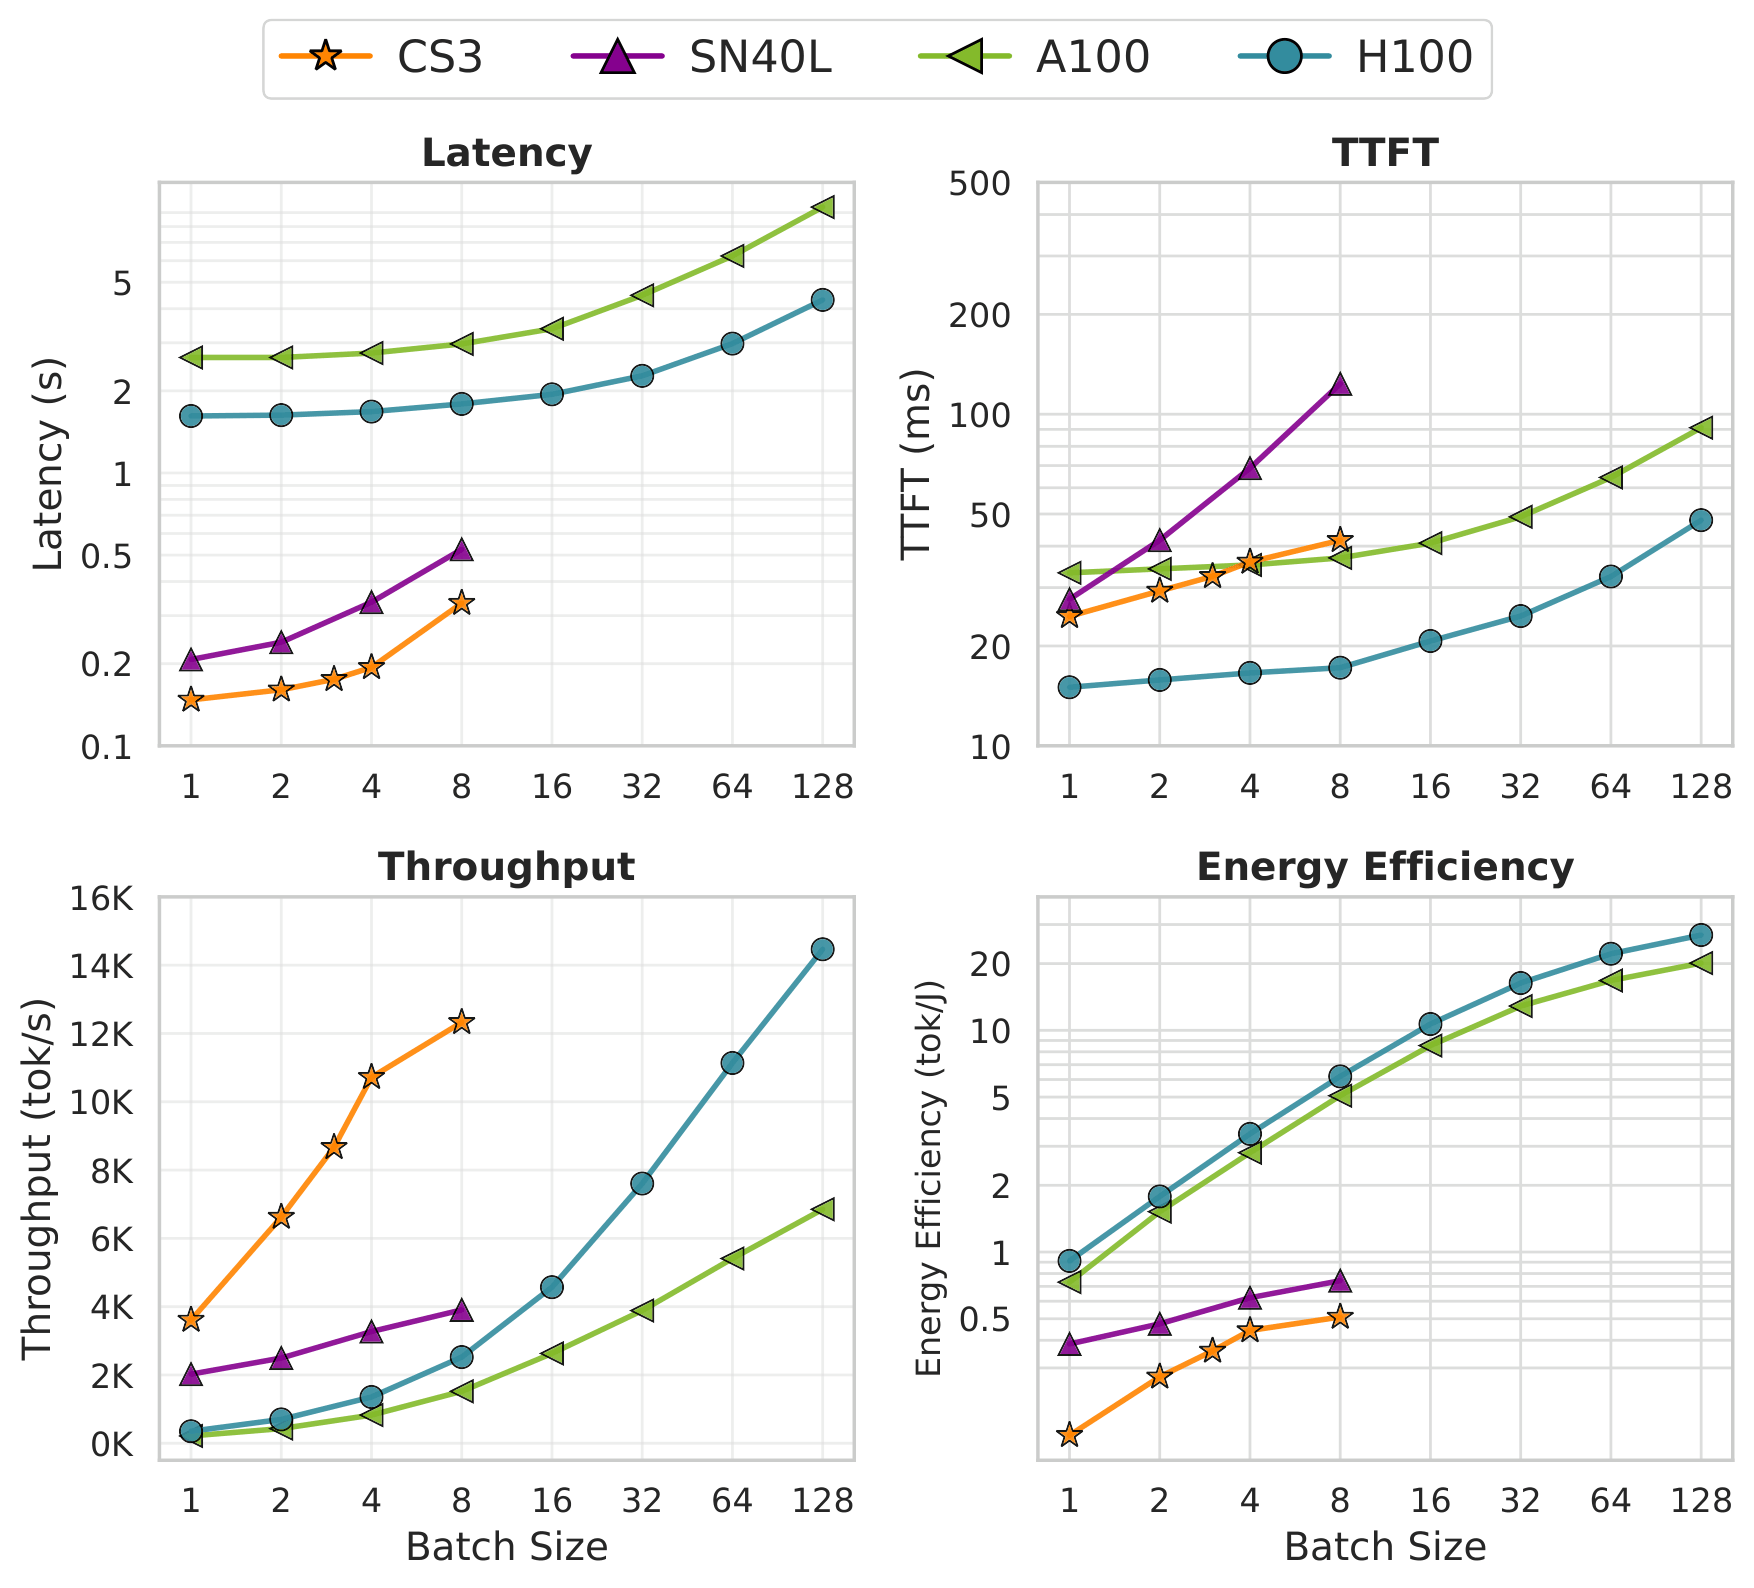
\includegraphics[width=0.8\columnwidth]{figs/testbeds_8B.png}
    \caption{Performance and energy efficiency of Llama 3.1 8B inference across AI accelerators.}
    \tagpdfsetup{alttext={Performance and energy efficiency of Llama 3.1 8B inference across AI accelerators.}}
    \label{fig:testbeds8}
\end{figure}

\ref{fig:testbeds8} and~\ref{fig:testbeds70} present the performance and energy-efficiency results for GPUs and dataflow accelerators running Llama~3.1~8B and Llama~3.3~70B, respectively, reporting four key metrics that highlight the differences in performance between GPUs and dataflow accelerators.

\begin{figure}[h!]
    \centering
    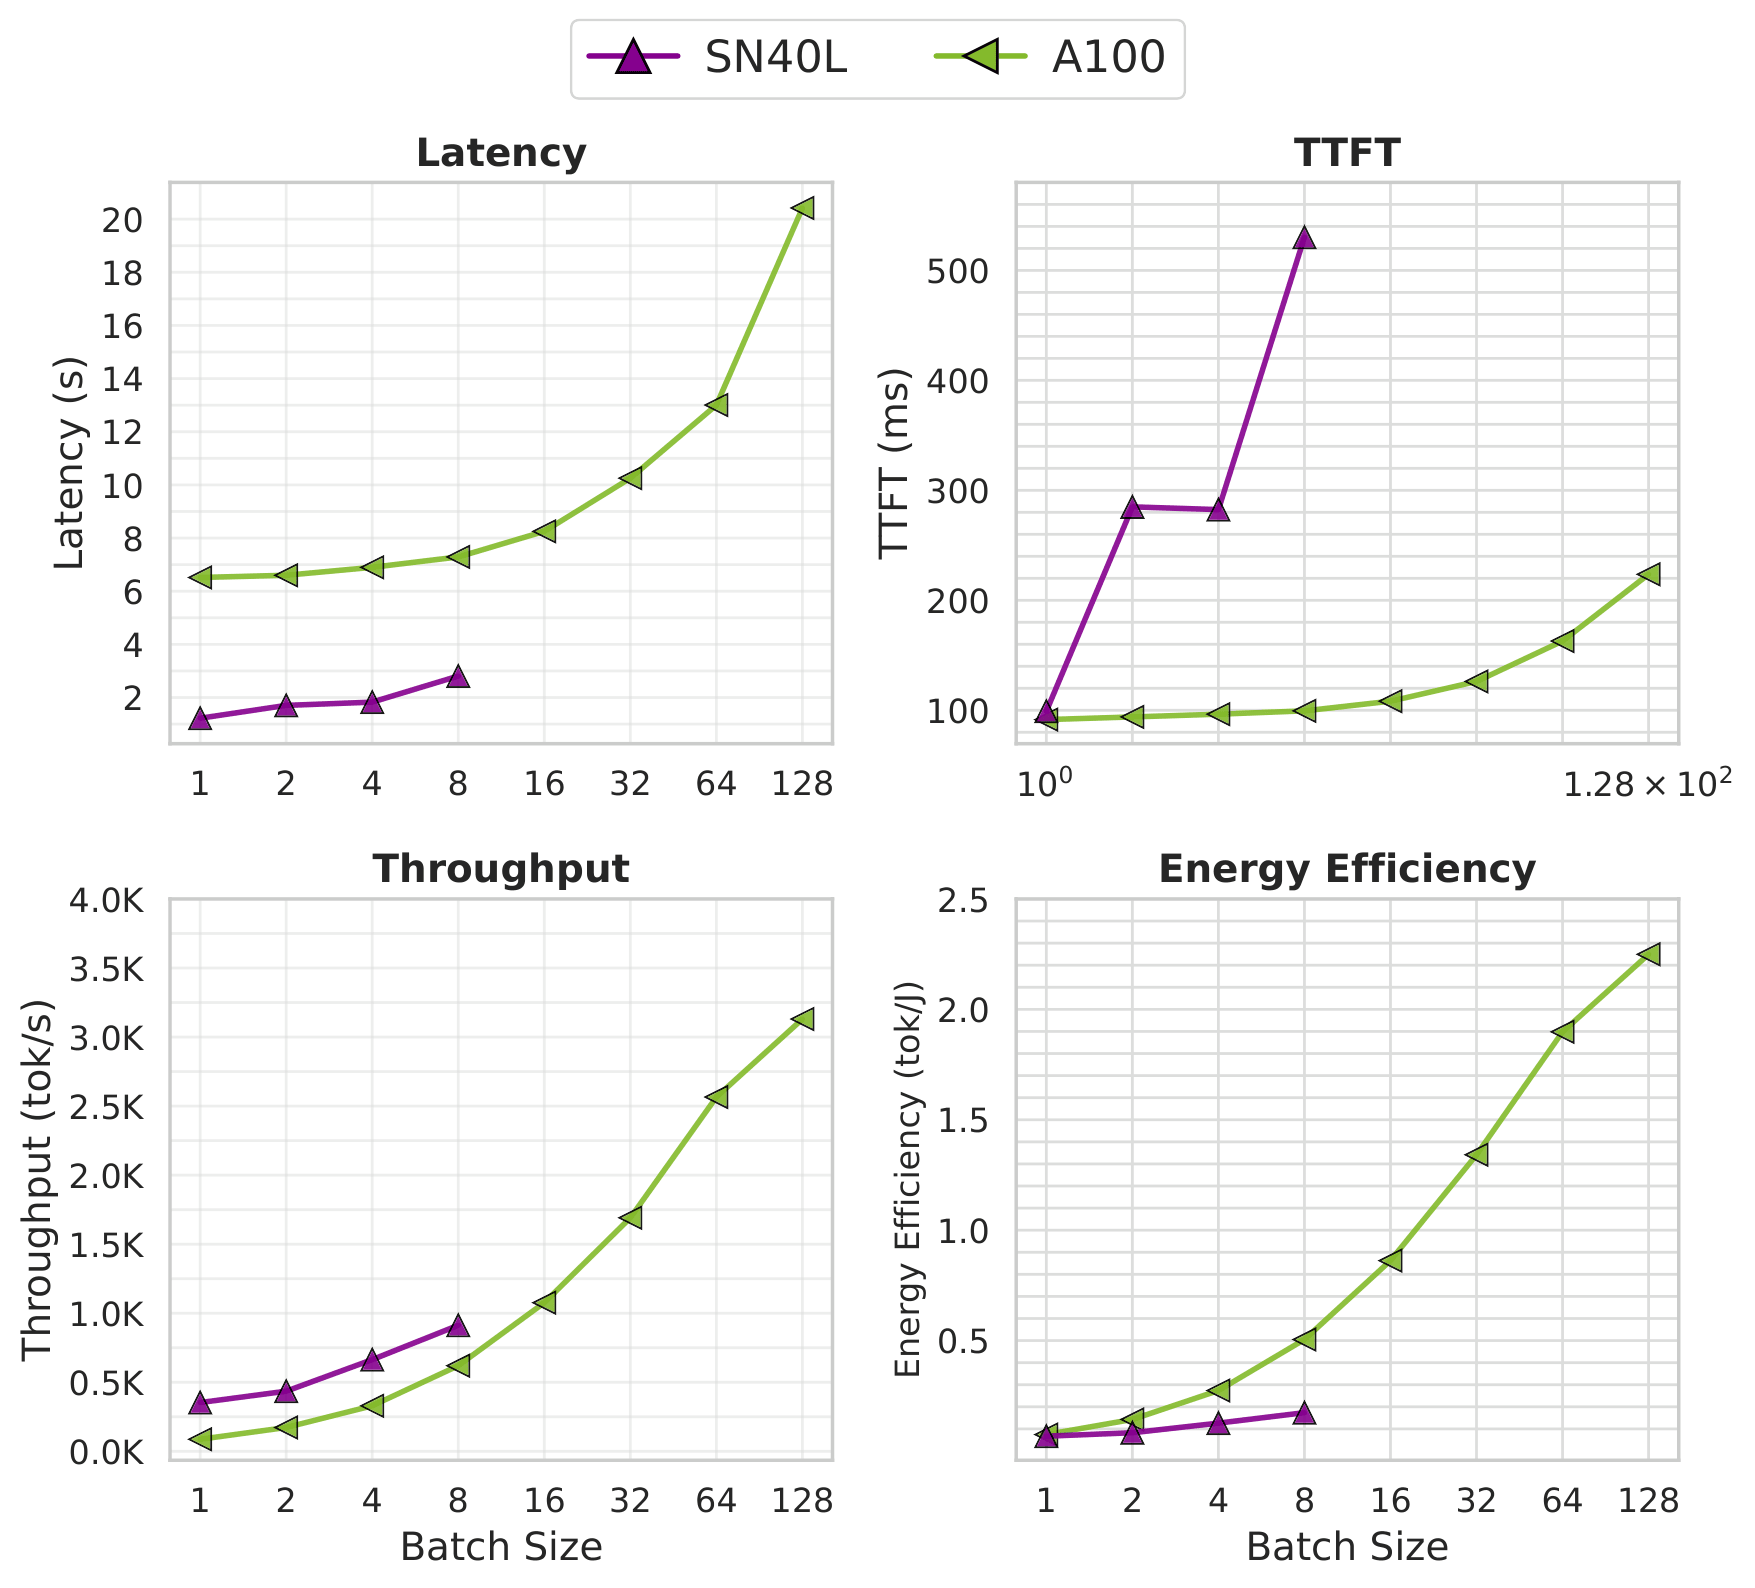
\includegraphics[width=0.8\columnwidth]{figs/testbeds_70.png}
      \caption{Performance and energy efficiency of Llama 3.3 70B inference across AI accelerators.}
    \tagpdfsetup{alttext={Performance and energy efficiency of Llama 3.3 70B inference across AI accelerators.}}
    \label{fig:testbeds70}
\end{figure}

Our experimental data clearly demonstrate how different architectures impact computation. As extensively discussed in Section \ref{chap:methods:sec:model}, LLM inference performance is directly related to the latency of the forward pass, which is composed of two parts: the latency of the computation and the latency of memory loading operations. GPUs host the model weights in off-chip HBM memories, which provide a bandwidth of approximately 1 to 5 TB/s. Dataflow accelerators, on the other hand, rely on local scratchpad memories, which are up to four orders of magnitude faster than GPUs, aiming to alleviate the impact of memory reads on the overall performance.
fi
At first, we observe that within their supported batch sizes, dataflow machines achieve markedly lower latency and substantially higher throughput than GPUs. The most pronounced improvement occurs at batch size 1, where the computation is the most memory-bound.
NVIDIA A100 reaches 215 tokens/s, compared to 3609 tokens/s (16.8$\times$) on the Cerebras CS3 and 2024 tokens/s (9.41$\times$) on the SambaNova SN40L.
The SamabaNova SN40L also outpaces GPUs with Llama 3.3 70B, achieving 353 tokens/s at a batch size of 1, compared to 88 tokens/s (4.01$\times$) obtained with 4 NVIDIA A100s working with Tensor Parallelism.

Increasing the batch size also increases the operational intensity $OI$, allowing GPUs to progressively close the GAP. In their supported batch size range (1-8), dataflow accelerators still outpace GPUs in terms of latency and throughput. However, due to the larger impact of computation on overall latency, we notice that dataflow accelerators display notably steeper increases in end-to-end latency and TTFT compared to those of GPUs.

Another observation regards peak throughput.
We established that dataflow machines exhibit superior performance at small batch sizes, but we also assessed the fact that their maximum supported batch size is substantially lower, sometimes due to a lack of compile artifacts for larger batch size configurations. In fact, both Cerebras and SambaNova provide precompiled artifacts that allow running at fixed batch sizes of 1 to 8. vLLM, on the other hand, handles batch sizes dynamically, allowing us to test batch sizes up to 128.
In an offline scenario, where the maximum achievable throughput using the optimal batch size is the only relevant performance metric, we observe that the capacity of GPUs to scale to larger batch sizes allows them to narrow the performance gap in terms of peak throughput. Cerebras, at a batch size of 8, produces 12327 tokens/s, outperforming both the NVIDIA A100 and the AMD MI300x. However, it is still outperformed by the NVIDIA H100 at a batch size of 128, which achieves 14,455 tokens/s. The SambaNova SN40L instead peaks at 3,907 tokens/s with a batch size of 8.
From this, we can conclude that the performance benefits of modern dataflow accelerators are noticeable, particularly in online settings with low batch sizes and a limited number of requests per node. In offline batch-inference jobs, the dynamic batch size supported by GPUs makes this architecture still preferred.

This causes dataflow accelerators to dominate online inference scenarios with a reduced number of concurrent requests, while in an online scenario where the only requirement is high throughput, they lose their competitive advantage in terms of raw performance.

\subsection{Comparison of ITL and TTFT}

\begin{figure}[h!]
    \centering
    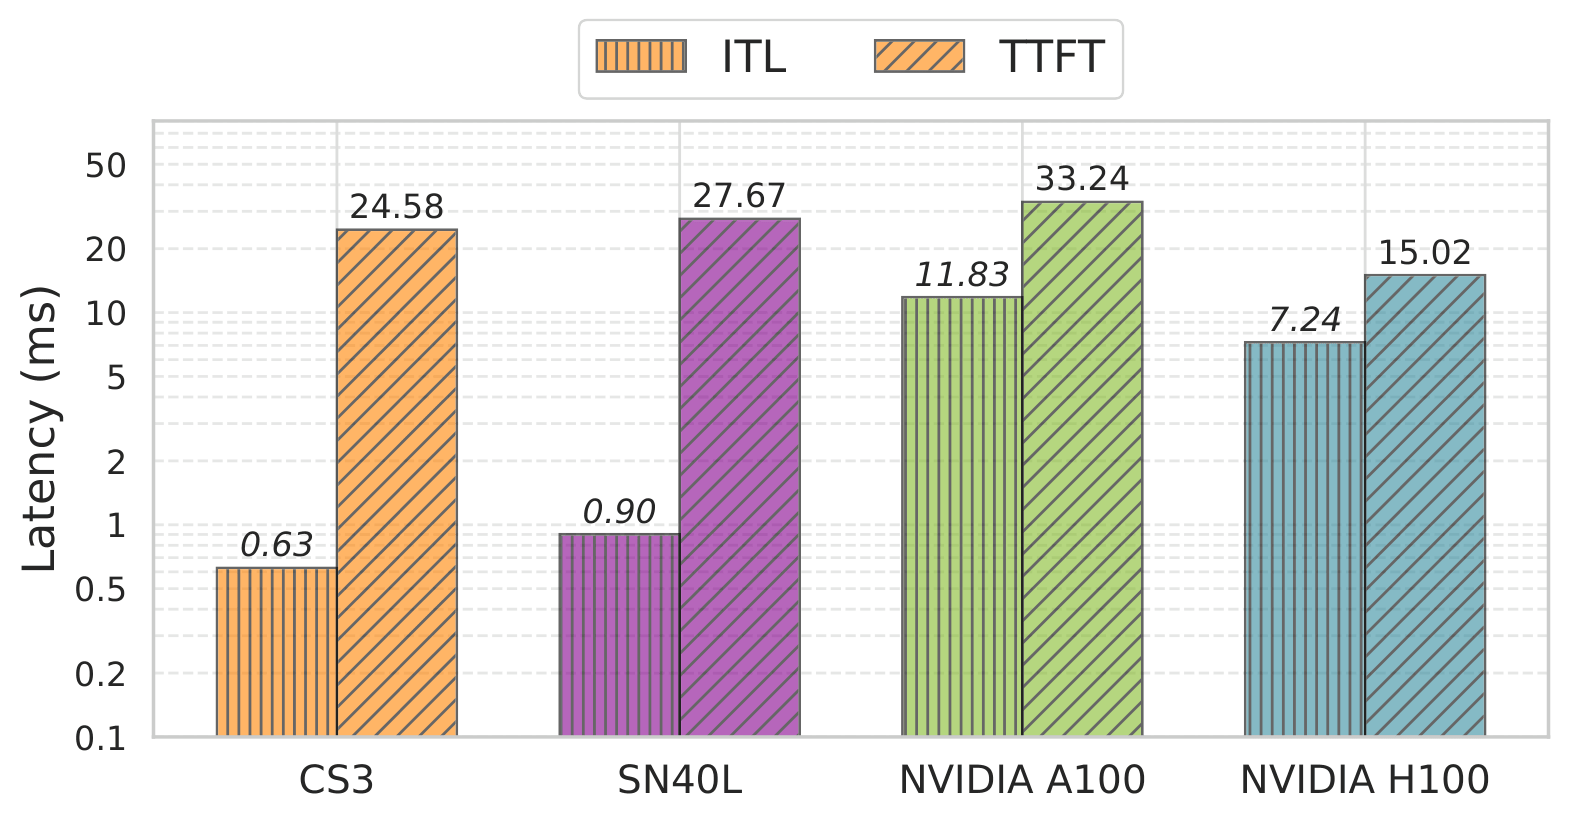
\includegraphics[width=\columnwidth]{figs/itl_ttft.png}
      \caption{Time-to-first-token (TTFT) and Inter Token Latency (ITL) of GPUs and dataflow accelerators.}
      \tagpdfsetup{alttext={Time-to-first-token (TTFT) and Inter Token Latency (ITL) of GPUs and dataflow accelerators.}}
    \label{fig:itl-ttft}
\end{figure}

Digging further into the impact of memory bandwidth on computation, we compare the ITL and TTFT across the different architectures. As discussed in \ref{chap:methods:sec:metrics}, TTFT is the average latency of the compute-bound prefill phase, while ITL indicates the average latency of the memory-bound decode phase.
\ref{fig:itl-ttft} displays TTFT and ITL of Llama 3.1 8B at batch size 1.
It allows us to observe once again how the benefit of dataflow accelerators stems from their improved data locality and memory bandwidth. In fact, while the TTFT of the SambaNova SN40L and the Cerebras CS3 is comparable with that of NVIDIA GPUs, the ITL is faster by one order of magnitude. Precisely, the Cerebras CS3 achieves an 18.8 $\times$ lower ITL compared to the NVIDIA A100, while SambaNova shows a 13.1 $\times$ improvement. A similar pattern appears when comparing Llama 3.3 70B performance: the SambaNova SN40L achieves slower TTFT compared to 4 NVIDIA A100 (99 ms compared to 91 ms), while having a 5.18 $\times$ shorter ITL (5.6 ms compared to 29 ms).

\subsection{Energy Efficiency}
\begin{figure}[H]
    \centering
    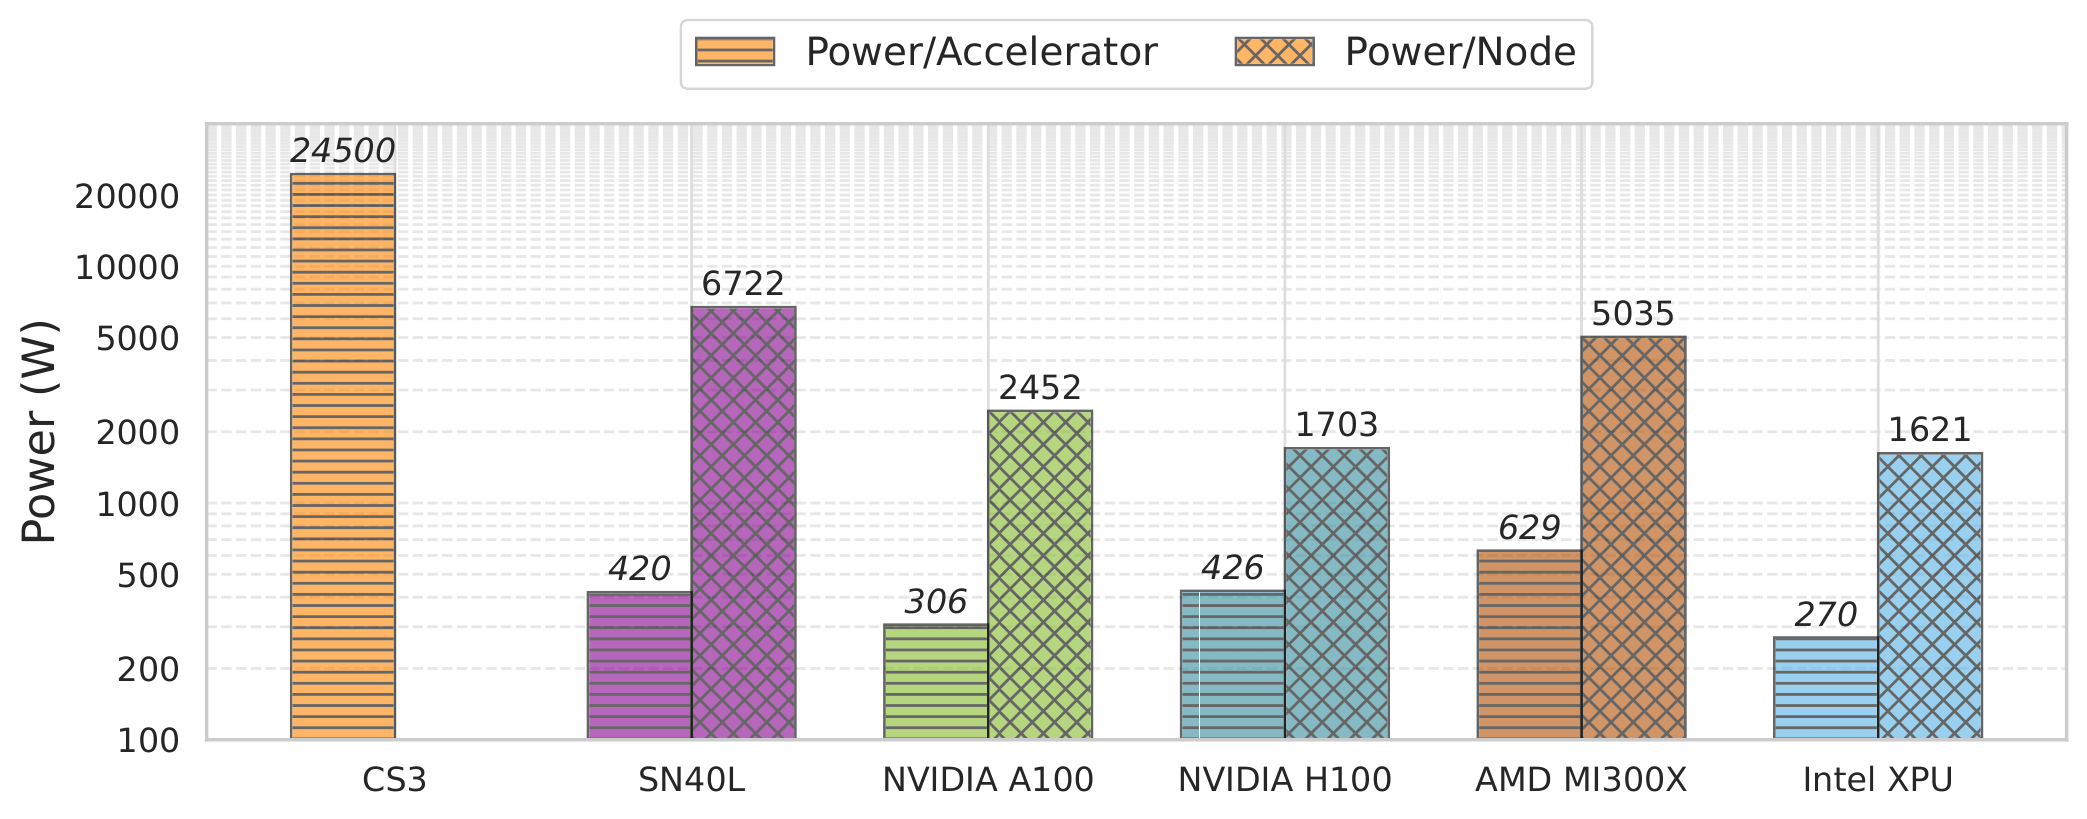
\includegraphics[width=\columnwidth]{figs/power_testbeds.png}
      \caption{Power consumption of GPUs and AI accelerators.}
      \tagpdfsetup{alttext={Power consumption of GPUs and AI accelerators.}}
    \label{fig:power}
\end{figure}

Finally, we analyze energy efficiency. To benefit from reduced memory bandwidth, dataflow accelerators employ a substantially larger number of cores that store weights and activations in their local memory, resulting in higher overall power consumption. As shown in \ref{fig:power}, to run Llama 3.1 8B in half precision, Cerebras CS3 draws around 24500W of power, and the SambaNova SN40L uses 420W per RDU, for a total of 6722W for the whole SN40L-16R system. Compared to the multi-GPU nodes, we observe that for the same model at a batch size of 16, GPUs use between 306 W and 630W of power.

For this reason, at no batch size, dataflow accelerators exhibit competitive energy consumption compared to GPUs (as shown in \ref{fig:testbeds8} and \ref{fig:testbeds70}), even though they display substantially better performance.

For this reason, we can conclude that a trade-off exists between low-latency, throughput, and energy efficiency among different types of accelerators.
